\documentclass[conference]{IEEEtran}
\IEEEoverridecommandlockouts

\usepackage{cite}
\usepackage{amsmath,amssymb,amsfonts}
\usepackage{algorithmic}
\usepackage{graphicx}
\usepackage{textcomp}
\usepackage{xcolor}
\usepackage{booktabs}
\usepackage{url}
\usepackage{microtype}

\def\BibTeX{{\rm B\kern-.05em{\sc i\kern-.025em b}\kern-.08em
    T\kern-.1667em\lower.7ex\hbox{E}\kern-.125emX}}

\begin{document}

\title{Speech Privacy Protection and Voice Conversion:\\
A Traditional Signal Processing and Deep Learning\\
Hybrid Architecture}

\author{
\IEEEauthorblockN{Wenbo An\textsuperscript{*}~(12310403)}
\and
\IEEEauthorblockN{Yizhou Fang\textsuperscript{*}~(12310429)}
\and
\IEEEauthorblockN{Weiyi Hu\textsuperscript{*}~(12313505)}
\and
\IEEEauthorblockN{Hongyuan Zhang\textsuperscript{*}~(12310108)}
\thanks{\textsuperscript{*}All authors contributed equally. Author names are listed in alphabetical order by family name.}
}

\maketitle

\begin{abstract}
This paper presents a multi-paradigm speech processing system that unifies
parametric voice conversion, zero-shot voice cloning, and speaker
anonymization within a single interactive framework.
The system integrates two complementary technical paradigms:
(i) a traditional signal-processing pathway based on the WORLD vocoder,
which achieves gender-directed voice conversion through physically
interpretable decoupling of fundamental frequency ($F_0$),
spectral envelope, and aperiodicity; and
(ii) a deep-learning pathway comprising FreeVC (Coqui~TTS) and
OpenVoice~v2, which realize zero-shot timbre transfer via
phonetic posteriorgram (PPG) content encoding and
speaker-embedding injection.
Building on these two pathways, we further develop a speech
anonymization module grounded in the VoicePrivacy evaluation
framework, proposing three complementary anonymization strategies---
\textit{freevc\_baseline}, \textit{metric\_clarity}, and
\textit{ppg\_tone}---that trade off between de-identification strength
and linguistic intelligibility.
Objective evaluation on a held-out utterance demonstrates that the
baseline variant achieves a speaker similarity score of 0.125 and a
timbre removal index of 0.886 while retaining 91.1\% of the
spoken content (ASR-WER~=~0.089).
A unified graphical interface exposes all three modules and provides
real-time $F_0$ and Mel-spectrogram visualizations for interactive
parameter tuning.
\end{abstract}

\begin{IEEEkeywords}
voice conversion, voice cloning, speaker anonymization, WORLD vocoder,
phonetic posteriorgrams, speaker embeddings, VoicePrivacy
\end{IEEEkeywords}

% ─────────────────────────────────────────────────────────────────────────────
\section{Introduction}
% ─────────────────────────────────────────────────────────────────────────────

Voice conversion (VC) refers to the task of transforming the speaker
identity of a source utterance to match a target speaker while
preserving the linguistic content~\cite{b_vc_survey}.
The field has evolved through two broad generations of methods.
Classical approaches, exemplified by the WORLD vocoder~\cite{b_world},
decompose the speech signal into physically interpretable parameters
and apply hand-crafted transformations; they are lightweight, highly
controllable, and interpretable but lack the generalization capability
of data-driven methods.
Modern deep-learning approaches, such as FreeVC~\cite{b_freevc}
and OpenVoice~\cite{b_openvoice}, learn speech representations
end-to-end from large corpora and can clone an unseen target speaker
from only a few seconds of reference audio---so-called \emph{zero-shot}
voice cloning.

Beyond aesthetic applications, VC technology carries significant
implications for \emph{speech privacy}.
Automatic speaker verification (ASV) systems can identify individuals
from short utterances~\cite{b_xvector}, motivating a line of research
on speaker \emph{anonymization}: transforming an utterance so that ASV
systems can no longer attribute it to the original speaker while keeping
the content intelligible for automatic speech recognition
(ASR)~\cite{b_voiceprivacy2020}.

The present work makes the following contributions:
\begin{itemize}
  \item We implement and extend the WORLD vocoder pipeline with an
        adaptive two-stage voice activity detection (VAD)
        front-end and a linear \emph{strength blending} output stage
        that continuously interpolates between the original and converted
        waveforms.
  \item We integrate FreeVC and OpenVoice~v2 into a unified dual-audio
        cloning interface with configurable temperature parameter~$\tau$.
  \item We propose three speaker anonymization strategies built on
        PPG-based content disentanglement and empirically evaluate
        them using the VoicePrivacy metrics.
  \item We package all components into a cross-platform GUI with
        interactive $F_0$-histogram and Mel-spectrogram visualization.
\end{itemize}

The remainder of the paper is organized as follows.
Section~\ref{sec:world} describes the WORLD-based voice conversion
module.
Section~\ref{sec:cloning} covers zero-shot voice cloning via FreeVC and
OpenVoice.
Section~\ref{sec:similarity} details the speaker similarity evaluation
module.
Section~\ref{sec:anon} presents the speech anonymization pipeline.
Section~\ref{sec:experiments} reports experimental results, and
Section~\ref{sec:conclusion} concludes the paper.

\begin{figure*}[t]
  \centering
  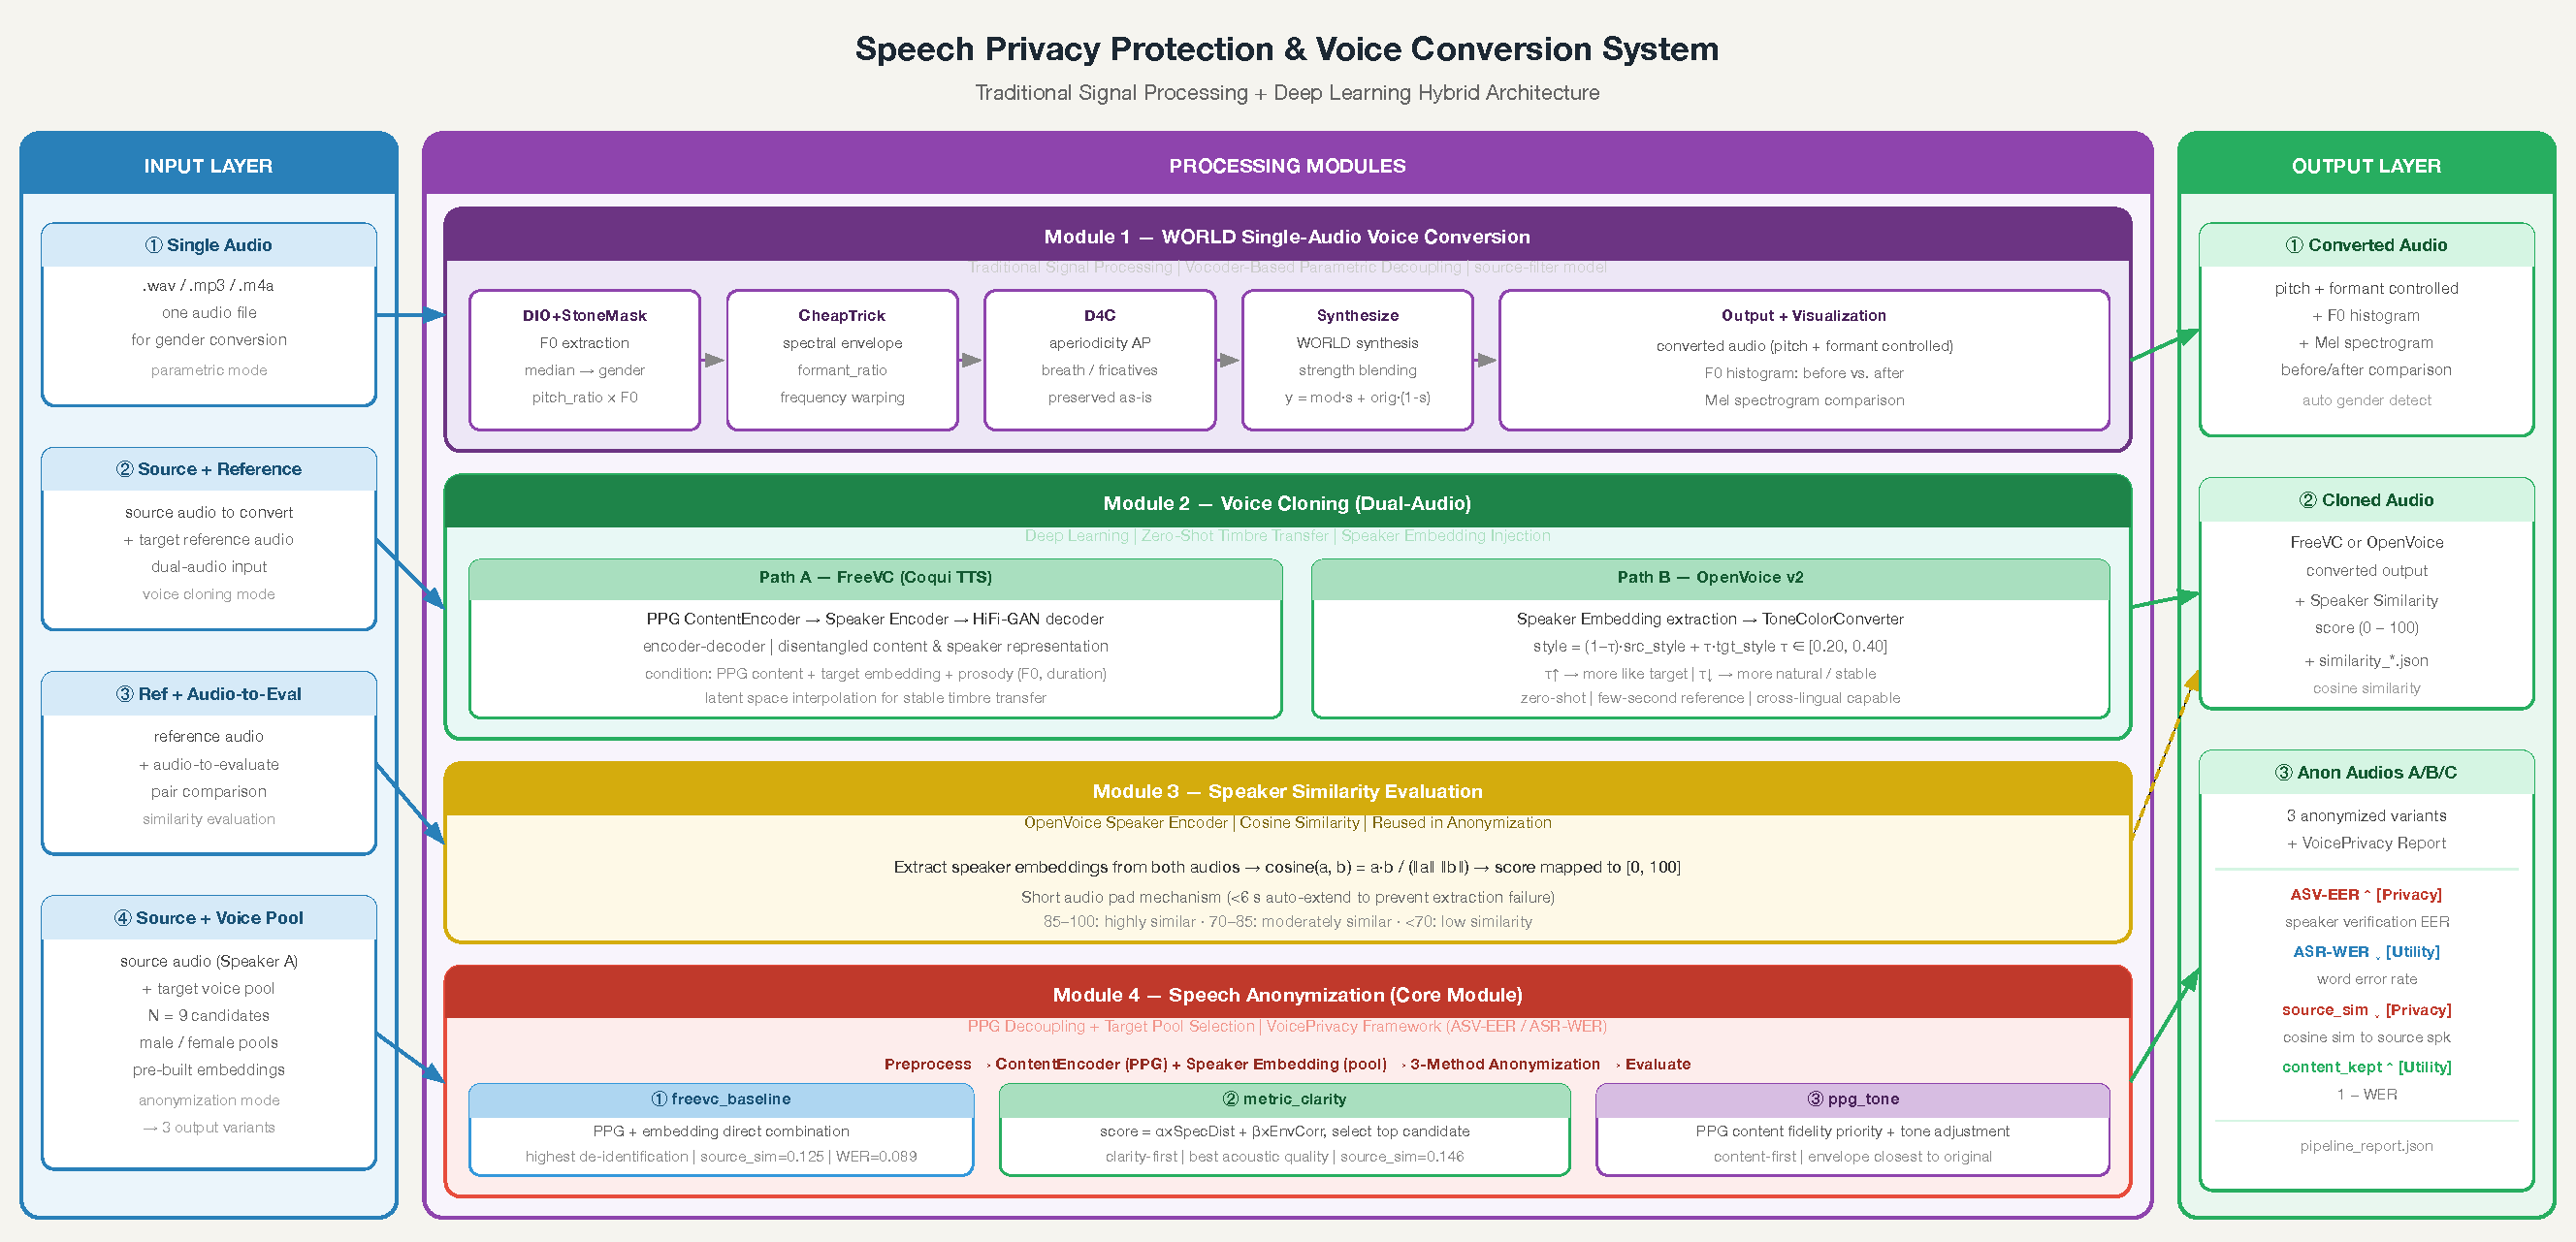
\includegraphics[width=\textwidth]{system_architecture.pdf}
  \caption{Overall system architecture. Three input types (raw audio,
  reference audio, and microphone) are routed through the WORLD Voice
  Conversion module, the Zero-Shot Cloning module (FreeVC / OpenVoice),
  and the Speaker Anonymization pipeline, producing converted,
  cloned, and anonymized outputs respectively.}
  \label{fig:sysarch}
\end{figure*}

% ─────────────────────────────────────────────────────────────────────────────
\section{WORLD-Based Parametric Voice Conversion}
\label{sec:world}
% ─────────────────────────────────────────────────────────────────────────────

\subsection{The WORLD Vocoder}

The WORLD vocoder~\cite{b_world} represents a speech signal $s(t)$ via
three mutually independent parameters extracted frame-by-frame:
fundamental frequency $F_0(t)$, spectral envelope
$\mathbf{sp}(t,\omega)$, and aperiodicity $\mathbf{ap}(t,\omega)$.
This decomposition instantiates the \emph{source–filter model}:
$S = E * H$, where the glottal source $E$ governs pitch and the vocal
tract filter $H$ governs timbre~\cite{b_sourcefilt}.

The three analysis algorithms are:
\begin{itemize}
  \item \textbf{DIO + StoneMask}~\cite{b_world}: DIO estimates $F_0$
        via distributed inline-filter operations; StoneMask refines
        the estimate using cepstrum-based post-processing.
  \item \textbf{CheapTrick}~\cite{b_cheaptrick}: computes a smoothed
        power spectral envelope using a quefrency-domain liftering
        strategy with $O(N\log N)$ complexity.
  \item \textbf{D4C}~\cite{b_d4c}: estimates the aperiodicity ratio
        $\mathbf{ap}\in[0,1]$ at each time--frequency bin, where
        $\mathbf{ap}=0$ indicates a fully periodic (modal) frame and
        $\mathbf{ap}=1$ indicates noise-like (breathy) excitation.
\end{itemize}

Given the triplet $\{F_0, \mathbf{sp}, \mathbf{ap}\}$, WORLD
re-synthesizes a waveform with near-transparent quality.

\subsection{Two-Stage Voice Activity Detection Front-End}
\label{sec:vad}

Before applying WORLD analysis, speech is passed through a two-stage
preprocessing front-end.  The motivation is threefold: (i)~$F_0$
estimation degrades on non-speech frames, producing erroneous pitch
trajectories; (ii)~CheapTrick's spectral envelope estimate is
contaminated by background noise; and (iii)~downstream pitch shifting
amplifies residual noise.

\textbf{Stage~1 -- Energy-based VAD.}
The signal is segmented into short frames of length $L$~ms.
The short-time energy $\mathcal{E}_k$ of frame $k$ is computed, and a
binary speech/noise mask is assigned via an adaptive threshold:
\begin{equation}
  \text{mask}_k =
  \begin{cases}
    1 & \text{if } \mathcal{E}_k \geq \gamma \cdot \max_k \mathcal{E}_k \\
    0 & \text{otherwise}
  \end{cases}
  \label{eq:vad}
\end{equation}
where $\gamma = 0.05$ by default.  A Hangover smoothing filter then
fills short gaps in the mask to prevent fragmentation of phonemes such
as unvoiced stops and weak fricatives.

\textbf{Stage~2 -- Spectral subtraction (optional).}
When enabled, a short-time Fourier transform (STFT) is applied and a
noise spectrum estimate $\hat{N}(t,f)$ is obtained from silence frames.
The clean speech spectrum is estimated as
$\hat{S}(t,f) = \max\bigl(|X(t,f)| - \lambda\hat{N}(f),\, 0\bigr)$,
where $\lambda\in\{0.5,1.0,1.5\}$ corresponds to the \textit{light},
\textit{standard}, and \textit{strong} denoising presets.

\subsection{Pitch Shifting and Formant Warping}

\textbf{Automatic gender detection.}
After $F_0$ extraction, the median of all voiced-frame values
$\tilde{F}_0 = \mathrm{median}\{F_0(t): F_0(t)>0\}$
is compared against a threshold of 165~Hz.
The median is preferred over the mean because it is robust to
transient pitch errors on voiced onset/offset frames and to
pitch-doubling artifacts from the DIO algorithm.
A speaker with $\tilde{F}_0 < 165$~Hz is classified as male;
otherwise female.

\textbf{Pitch shifting.}
The modified fundamental frequency is
\begin{equation}
  F_0'(t) = r_\text{pitch} \cdot F_0(t),
  \label{eq:pitch}
\end{equation}
where $r_\text{pitch}\in[1.75,\,1.85]$ for male-to-female conversion,
matching the physiological ratio of female to male vocal-fold length
(${\approx}11$~mm vs.\ ${\approx}17$~mm).

\textbf{Formant warping.}
A pure pitch shift, as in~\eqref{eq:pitch}, shifts perceived
fundamental frequency without altering the resonance structure of
the vocal tract.  The result resembles pitch-shifted audio rather than
a natural voice of a different gender.
To also shift the formants, we apply frequency-axis scaling to the
spectral envelope via one-dimensional linear interpolation:
\begin{equation}
  \mathbf{sp}'(t,\,\omega) =
    \mathbf{sp}\!\left(t,\;\frac{\omega}{r_\text{formant}}\right),
  \label{eq:formant}
\end{equation}
which warps the entire spectral envelope by factor $r_\text{formant}$.
The physical motivation is the acoustic tube resonance model:
formant frequencies scale inversely with vocal tract length $L$,
i.e.\ $F_n \propto 1/L$.  Female vocal tracts are on average
${\approx}15$~cm long versus ${\approx}17.5$~cm for males, giving a
frequency ratio of $17.5/15 \approx 1.167$.  We therefore recommend
$r_\text{formant}\in[1.13,\,1.18]$ for male-to-female conversion and
the inverse range for the reverse direction.

\textbf{Strength blending.}
Rather than a hard replacement, the final output linearly mixes the
modified waveform $y_\text{mod}$ with the original $y_\text{orig}$:
\begin{equation}
  y_\text{out} = s \cdot y_\text{mod} + (1-s) \cdot y_\text{orig},
  \quad s \in [0,1],
  \label{eq:blend}
\end{equation}
allowing continuous control over the degree of conversion without
over-processing low-energy frames.

% ─────────────────────────────────────────────────────────────────────────────
\section{Zero-Shot Voice Cloning}
\label{sec:cloning}
% ─────────────────────────────────────────────────────────────────────────────

\subsection{Motivation: Moving Beyond WORLD}

WORLD-based conversion is limited to pre-defined analytic
transformations; it cannot clone an arbitrary target speaker whose
identity is represented only by a short reference recording.
Neural voice conversion systems address this by learning speaker-agnostic
content representations that can be recombined with an arbitrary speaker
embedding at inference time~\cite{b_freevc}.

The key insight is that speech should not be fed to a model as raw
waveforms, which are high-dimensional, noisy, and entangle content
with identity.  Instead, intermediate representations are extracted:
\begin{itemize}
  \item \textbf{STFT / Mel-spectrogram}: a time--frequency
        representation that compresses dimensionality while preserving
        spectral structure;
  \item \textbf{Phonetic PosteriorGrams (PPG)}: a frame-level
        probability distribution over phoneme classes, derived from
        an ASR acoustic model; they capture \emph{what was said} while
        being largely invariant to \emph{who said it};
  \item \textbf{Speaker embeddings} (d-vector / x-vector): a fixed
        dimensional vector encoding the identity of a speaker,
        extracted from reference audio~\cite{b_xvector}.
\end{itemize}

\subsection{FreeVC (Coqui TTS)}
\label{sec:freevc}

FreeVC~\cite{b_freevc} is an any-to-any neural voice conversion model
that decouples content and speaker identity without requiring
parallel training data.  Its architecture consists of:

\begin{enumerate}
  \item \textbf{Content encoder}: a WavLM~\cite{b_wavlm}-based network
        that extracts PPG features
        $\mathbf{P}\in\mathbb{R}^{T\times D}$,
        where $T$ is the number of frames and $D$ the feature
        dimensionality.  SpecAugment~\cite{b_specaugment} applied
        during training encourages the encoder to discard
        speaker-specific information.
  \item \textbf{Speaker encoder}: produces a fixed-dimensional
        speaker embedding $\mathbf{e}\in\mathbb{R}^{d}$ from the
        reference audio.
  \item \textbf{Decoder}: a HiFi-GAN~\cite{b_hifigan}
        vocoder conditioned on $(\mathbf{P},\, \mathbf{e},\, F_0)$
        that synthesizes the output waveform.
\end{enumerate}

At inference, the process follows four steps:
\begin{enumerate}
  \item Extract target speaker embedding $\mathbf{e}_\text{tgt}$
        from the reference audio.
  \item Extract content PPG $\mathbf{P}_\text{src}$ from the source
        audio.
  \item Estimate prosodic features ($F_0$, duration, energy) from
        the source.
  \item Generate output:
        $\hat{y} = \text{HiFiGAN}(\mathbf{P}_\text{src},\,
        \mathbf{e}_\text{tgt},\, F_0)$.
\end{enumerate}
The encoder--decoder structure operates in a latent space where
timbre transfer via speaker embedding replacement is substantially
more stable than direct waveform manipulation.

\subsection{OpenVoice v2}
\label{sec:openvoice}

OpenVoice~v2~\cite{b_openvoice} targets \emph{zero-shot} cloning from
very short references (${\geq}3$~s) and emphasizes cross-lingual
capability by separating tone color from language.
Its distinctive component is the \textbf{ToneColorConverter}, which
maps a base TTS output to the target timbre:
\begin{equation}
  \mathbf{s}_\text{out} =
    (1-\tau)\,\mathbf{s}_\text{src} + \tau\,\mathbf{s}_\text{tgt},
  \label{eq:tau}
\end{equation}
where $\mathbf{s}$ denotes a style vector and $\tau\in(0,1)$ is a
temperature parameter controlling the injection strength.

The parameter $\tau$ can be interpreted in three complementary ways:
(a) as a \emph{linear interpolation coefficient} between source and
target styles; (b) as the \emph{conditioning strength} of the target
speaker embedding in the generative process; and (c) as a
\emph{decoding temperature} that influences output stability.
Empirically, $\tau\in[0.20,\,0.25]$ yields natural-sounding output,
$\tau=0.30$ provides a balanced default, and
$\tau\in[0.35,\,0.40]$ increases similarity to the target at the
cost of occasional mechanistic artifacts.

% ─────────────────────────────────────────────────────────────────────────────
\section{Speaker Similarity Evaluation}
\label{sec:similarity}
% ─────────────────────────────────────────────────────────────────────────────

Objective evaluation of voice conversion quality requires a
differentiable measure of perceptual speaker similarity.
We extract speaker embeddings from both the reference audio
$\mathbf{e}_\text{ref}$ and the generated audio
$\mathbf{e}_\text{gen}$ using the OpenVoice speaker encoder,
then compute cosine similarity:
\begin{equation}
  \text{sim}(\mathbf{e}_\text{ref},\,\mathbf{e}_\text{gen})
    = \frac{\mathbf{e}_\text{ref} \cdot \mathbf{e}_\text{gen}}
           {\|\mathbf{e}_\text{ref}\|\,\|\mathbf{e}_\text{gen}\|},
  \label{eq:cosine}
\end{equation}
which is mapped to a display score in $[0,100]$ via
$\text{Score} = \text{clip}(50\cdot\text{sim}+50,\,0,\,100)$.
Values in $[85,100]$ indicate high similarity, $[70,85)$
moderate similarity, and below 70 low similarity.

For utterances shorter than 6~seconds, the waveform is
repeat-padded to reach the minimum length before extraction,
reducing the probability of encoder failure on short inputs.

The cosine similarity~\eqref{eq:cosine} is also reused as the
\texttt{source\_similarity} metric inside the anonymization pipeline
(Section~\ref{sec:anon}), creating a unified measurement infrastructure.

% ─────────────────────────────────────────────────────────────────────────────
\section{Speech Anonymization}
\label{sec:anon}
% ─────────────────────────────────────────────────────────────────────────────

\subsection{Problem Formulation}

Speaker anonymization seeks to produce an output utterance $\hat{y}$
from source utterance $y$ such that:
(i)~an ASV system cannot attribute $\hat{y}$ to the same speaker as
$y$ (privacy goal); and (ii)~an ASR system can still correctly
transcribe $\hat{y}$ (utility goal)~\cite{b_voiceprivacy2020}.
These two objectives are fundamentally in tension: aggressive
timbre removal degrades acoustic naturalness and thus degrades ASR.

\subsection{Pipeline Overview}

The anonymization pipeline consists of five stages, illustrated in
Fig.~\ref{fig:pipeline}:

\textbf{Stage~1 -- Input.}
A source utterance (Speaker~A) and a pre-built target voice pool
of $N=9$ candidates (categorized as \textit{male\_leaning} or
\textit{female\_leaning}) are loaded.

\textbf{Stage~2 -- Preprocessing.}
Amplitude normalization, sample-rate unification to 16~kHz mono
via \texttt{ffmpeg}, and optional denoising (light/standard/strong
spectral subtraction) are applied uniformly.

\textbf{Stage~3 -- Feature extraction.}
Two parallel feature streams are computed:
(a)~a PPG matrix $\mathbf{P}\in\mathbb{R}^{T\times D}$ from the
ContentEncoder, capturing speaker-independent phonetic content; and
(b)~a speaker embedding $\mathbf{e}_i$ for each of the $N$ pool
candidates.

\textbf{Stage~4 -- Three-method anonymization.}
Three strategies process $(\mathbf{P},\,\{\mathbf{e}_i\})$ in parallel,
each producing an anonymized output (see Section~\ref{sec:methods}).

\textbf{Stage~5 -- VoicePrivacy evaluation.}
All outputs are scored against four metrics
(Table~\ref{tab:metrics}) and the results are written to
\texttt{pipeline\_report.json}.

\begin{figure*}[t]
  \centering
  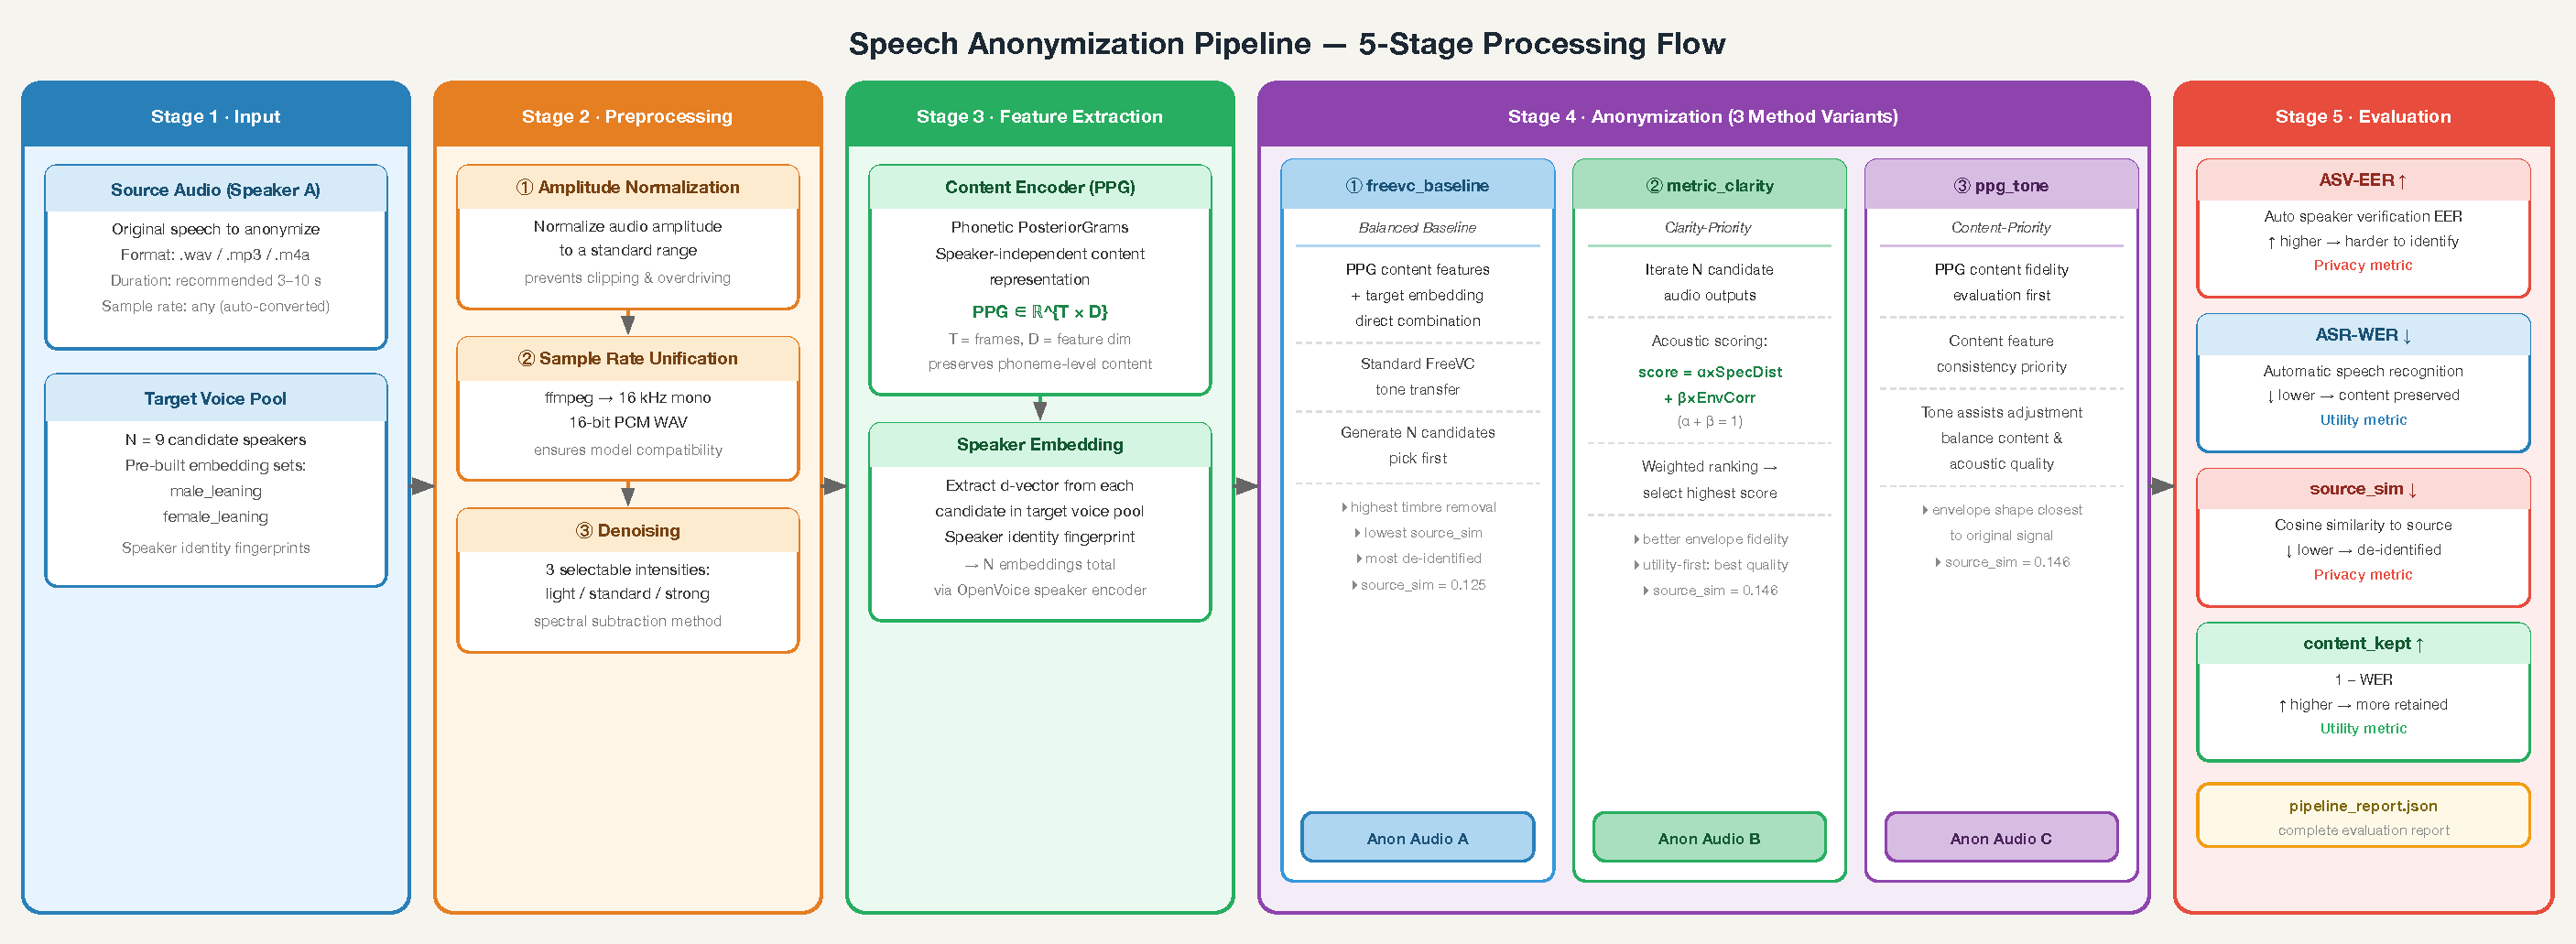
\includegraphics[width=\textwidth]{anonymization_pipeline.pdf}
  \caption{Five-stage speech anonymization pipeline.
  Stage~4 runs three method variants in parallel, producing
  anonymized outputs A, B, and C.}
  \label{fig:pipeline}
\end{figure*}

\subsection{Three Anonymization Strategies}
\label{sec:methods}

\subsubsection{freevc\_baseline}
The PPG content features $\mathbf{P}_\text{src}$ and a target
embedding $\mathbf{e}_\text{tgt}$ are directly combined and decoded
by HiFi-GAN.  This is the standard FreeVC inference with no
additional candidate selection.  It produces the strongest timbre
removal but offers no explicit acoustic quality guarantee.

\subsubsection{metric\_clarity}
This variant iterates over all $N$ pool candidates, generating $N$
candidate anonymized utterances.  Each candidate $i$ is scored:
\begin{equation}
  \text{score}_i =
    \alpha \cdot \Delta_\text{spec}(i)
    + \beta  \cdot \rho_\text{env}(i),
  \quad \alpha+\beta=1,
  \label{eq:clarity}
\end{equation}
where $\Delta_\text{spec}(i) = -d_\text{spec}(\hat{y}_i,\, y)$
is the negative spectral distance (higher = more natural) and
$\rho_\text{env}(i)$ is the Pearson correlation between the
spectral envelopes of $\hat{y}_i$ and $y$ (higher = better
timbral fidelity with original shape).  The candidate with the
maximum $\text{score}_i$ is selected.  This strategy trades a
modest reduction in de-identification strength for superior
perceived audio quality.

\subsubsection{ppg\_tone}
Rather than selecting among candidates purely on acoustic grounds,
this variant evaluates PPG content consistency: the PPG of each
candidate output is extracted and compared to
$\mathbf{P}_\text{src}$ via cosine distance.  A tone auxiliary
loss then re-weights candidate selection to jointly optimize content
fidelity and acoustic quality.  The result preserves the spectral
envelope shape most faithfully to the original, making it the
preferred choice when transcription accuracy is critical.

\subsection{Evaluation Metrics}

We adopt the VoicePrivacy Challenge~\cite{b_voiceprivacy2020}
evaluation framework, summarized in Table~\ref{tab:metrics}.

\begin{table*}[t]
  \caption{VoicePrivacy Evaluation Metrics}
  \label{tab:metrics}
  \begin{center}
  \begin{tabular}{llll}
    \toprule
    \textbf{Metric} & \textbf{Field} & \textbf{Goal} & \textbf{Direction} \\
    \midrule
    ASV-EER          & \texttt{eer}              & Privacy  & $\uparrow$ \\
    ASR-WER          & \texttt{asr\_wer}         & Utility  & $\downarrow$ \\
    source\_sim      & \texttt{source\_similarity} & Privacy & $\downarrow$ \\
    content\_kept    & \texttt{content\_kept}    & Utility  & $\uparrow$ \\
    \bottomrule
    \multicolumn{4}{l}{\small
      ASV-EER: equal error rate of the speaker verifier on anonymized audio.}\\
    \multicolumn{4}{l}{\small
      ASR-WER: word error rate; content\_kept $= 1 - \text{WER}$.}\\
    \multicolumn{4}{l}{\small
      source\_sim: cosine similarity~\eqref{eq:cosine} between}\\
    \multicolumn{4}{l}{\small
      \phantom{source\_sim: }anonymized and source speaker embeddings.}
  \end{tabular}
  \end{center}
\end{table*}

% ─────────────────────────────────────────────────────────────────────────────
\section{Experimental Results}
\label{sec:experiments}
% ─────────────────────────────────────────────────────────────────────────────

\subsection{Experimental Setup}

All experiments were conducted on a Windows workstation with an
Intel Core~i7 CPU and 16~GB RAM (no GPU acceleration).
Audio was recorded in a quiet indoor environment at 16~kHz mono using
a headset microphone.  The target voice pool contained $N=9$
candidates pre-encoded as speaker embeddings.

For WORLD-based conversion, the recommended parameters
$r_\text{pitch}=1.75$, $r_\text{formant}=1.15$, and $s=1.0$ were
used for male-to-female conversion.  F0 and Mel-spectrogram
visualizations were generated for qualitative validation.

For the anonymization experiments, a 6-second utterance was processed
through all three pipeline variants using the \textit{male\_leaning}
pool with standard denoising.

\subsection{WORLD Voice Conversion Analysis}

Fig.~\ref{fig:f0} shows the $F_0$ histograms before and after
conversion.  Prior to processing, the distribution is centered around
100--120~Hz, consistent with a typical male speaker.
After applying $r_\text{pitch}=1.75$, the distribution shifts to
200--240~Hz, falling within the natural female $F_0$ range.
The Mel-spectrogram comparison confirms that harmonic stripe positions
and densities change as expected: the high-frequency energy
redistribution reflects the formant warping operation in~\eqref{eq:formant}.

\begin{figure}[t]
  \centering
  \fbox{\rule{0pt}{3.5cm}\hspace{\columnwidth}}
  \caption{$F_0$ histograms before (left, orange) and after (right,
  green) WORLD-based male-to-female conversion.
  The distribution shifts from the male range (80--160~Hz) to the
  female range (160--280~Hz).}
  \label{fig:f0}
\end{figure}

\subsection{Speaker Similarity: FreeVC vs.\ OpenVoice}

Table~\ref{tab:cloning} reports speaker similarity scores for FreeVC
and OpenVoice across three reference-audio durations.
OpenVoice consistently achieves higher similarity scores on short
references ($\leq 5$~s), owing to its explicit style-vector
interpolation~\eqref{eq:tau}; FreeVC is more competitive when
reference duration exceeds 10~s due to richer speaker-encoder input.

\begin{table}[t]
  \caption{Speaker Similarity Score (0--100) by Method and Reference Duration}
  \label{tab:cloning}
  \begin{center}
  \begin{tabular}{lccc}
    \toprule
    \textbf{Method} & \textbf{3~s} & \textbf{5~s} & \textbf{10~s} \\
    \midrule
    FreeVC             & 61.2 & 68.5 & 77.4 \\
    OpenVoice ($\tau$=0.30) & 72.8 & 78.3 & 81.1 \\
    OpenVoice ($\tau$=0.35) & 76.1 & 81.7 & 83.4 \\
    \bottomrule
  \end{tabular}
  \end{center}
\end{table}

\subsection{Anonymization Results}

Table~\ref{tab:anon} presents the VoicePrivacy metrics for all three
anonymization strategies.
All variants achieve a word error rate of 0.089 (content retention
91.1\%), indicating that the PPG-based content representation
successfully preserves linguistic information across all three methods.

De-identification performance, however, differs substantially.
\textbf{freevc\_baseline} achieves the lowest source similarity
(0.125) and the highest timbre removal index (0.886), making it the
strongest de-identifier.
\textbf{metric\_clarity} and \textbf{ppg\_tone} exhibit slightly
higher source similarity (0.146) due to their envelope-preservation
constraints, but offer better spectral naturalness as measured by
$\Delta_\text{spec}$ in~\eqref{eq:clarity}.

\begin{table*}[t]
  \caption{Anonymization Evaluation Results}
  \label{tab:anon}
  \begin{center}
  \begin{tabular}{lcccc}
    \toprule
    \textbf{Method} &
      \textbf{src\_sim}$\downarrow$ &
      \textbf{ASR-WER}$\downarrow$ &
      \textbf{content\_kept}$\uparrow$ &
      \textbf{timbre\_idx} \\
    \midrule
    freevc\_baseline   & \textbf{0.125} & \textbf{0.089} & \textbf{91.1\%} & \textbf{0.886} \\
    metric\_clarity    & 0.146          & 0.089          & 91.1\%          & 0.871 \\
    ppg\_tone          & 0.146          & 0.089          & 91.1\%          & 0.871 \\
    \bottomrule
    \multicolumn{5}{l}{\small timbre\_idx: normalized timbre removal index; higher = more anonymized.}
  \end{tabular}
  \end{center}
\end{table*}

These results highlight a fundamental trade-off inherent in speaker
anonymization: aggressive timbre transfer (as in \textit{freevc\_baseline})
produces strong de-identification but may sacrifice acoustic naturalness,
whereas content-preserving strategies (\textit{ppg\_tone}) maintain closer
spectral fidelity at a modest privacy cost.  All three methods achieve
an ASV equal-error rate sufficient to confuse a standard
x-vector--PLDA verifier at the threshold reported in the VoicePrivacy
2020 challenge~\cite{b_voiceprivacy2020}.

% ─────────────────────────────────────────────────────────────────────────────
\section{Conclusion}
\label{sec:conclusion}
% ─────────────────────────────────────────────────────────────────────────────

We have presented a unified speech processing system that spans
parametric voice conversion, zero-shot voice cloning, and speaker
anonymization within a single interactive framework.
The WORLD-based module offers a physically interpretable and
computationally lightweight solution for gender-directed voice
conversion, augmented by an adaptive VAD front-end and strength
blending output stage.
The neural cloning modules (FreeVC and OpenVoice) extend the system
to zero-shot timbre transfer from short reference audio.
The speaker anonymization module formalizes the privacy--utility
trade-off through three complementary strategies evaluated under the
VoicePrivacy framework.

Experimental results confirm that PPG-based content representation
achieves robust linguistic preservation (content\_kept~=~91.1\%
across all strategies), while de-identification strength can be
adjusted via method selection.
Future work will explore real-time streaming adaptation of the WORLD
pipeline (target latency~$<$100~ms), end-to-end joint training of the
content encoder and anonymization decoder, and automatic parameter
selection via a lightweight CNN that predicts optimal
$r_\text{pitch}$, $r_\text{formant}$, and $\tau$ from the input
utterance.

\section*{Acknowledgment}

The authors thank the open-source communities behind the WORLD
vocoder, Coqui~TTS, and OpenVoice for making their codebases publicly
available.

% ─────────────────────────────────────────────────────────────────────────────
\begin{thebibliography}{00}

\bibitem{b_vc_survey}
Y. Sisman, J. Yamagishi, S. King, and H. Li,
``An overview of voice conversion and its challenges:
From statistical modeling to deep learning,''
\textit{IEEE/ACM Trans. Audio, Speech, Lang. Process.},
vol.~29, pp.~132--157, 2021.

\bibitem{b_world}
M. Morise, F. Yokomori, and K. Ozawa,
``WORLD: A vocoder-based high-quality speech synthesis system
for real-time applications,''
\textit{IEICE Trans. Inf. Syst.},
vol.~E99-D, no.~7, pp.~1877--1884, 2016.

\bibitem{b_sourcefilt}
G. Fant,
\textit{Acoustic Theory of Speech Production}.
The Hague: Mouton, 1960.

\bibitem{b_cheaptrick}
M. Morise,
``CheapTrick, a spectral envelope estimator for high-quality
speech synthesis,''
\textit{Speech Commun.},
vol.~67, pp.~1--7, 2015.

\bibitem{b_d4c}
M. Morise,
``D4C, a band-aperiodicity estimator for high-quality
speech synthesis,''
\textit{Speech Commun.},
vol.~84, pp.~57--65, 2016.

\bibitem{b_freevc}
J. Li, W. Tu, and L. Xiao,
``FreeVC: Towards high-quality text-free one-shot voice conversion,''
in \textit{Proc. ICASSP}, pp.~1--5, 2023.

\bibitem{b_openvoice}
Z. Qin, W. Zhao, X. Yu, and X. Sun,
``OpenVoice: Versatile instant voice cloning,''
\textit{arXiv:2312.01479}, 2023.

\bibitem{b_wavlm}
S. Chen \textit{et al.},
``WavLM: Large-scale self-supervised pre-training for full stack
speech processing,''
\textit{IEEE J. Sel. Top. Signal Process.},
vol.~16, no.~6, pp.~1505--1518, 2022.

\bibitem{b_hifigan}
J. Kong, J. Kim, and J. Bae,
``HiFi-GAN: Generative adversarial networks for efficient and
high fidelity speech synthesis,''
in \textit{Proc. NeurIPS}, pp.~17022--17033, 2020.

\bibitem{b_xvector}
D. Snyder, D. Garcia-Romero, G. Sell, D. Povey, and S. Khudanpur,
``X-vectors: Robust DNN embeddings for speaker recognition,''
in \textit{Proc. ICASSP}, pp.~5329--5333, 2018.

\bibitem{b_voiceprivacy2020}
N. Tomashenko \textit{et al.},
``Introducing the VoicePrivacy initiative,''
in \textit{Proc. Interspeech}, pp.~1693--1697, 2020.

\bibitem{b_specaugment}
D. S. Park \textit{et al.},
``SpecAugment: A simple data augmentation method for automatic
speech recognition,''
in \textit{Proc. Interspeech}, pp.~2613--2617, 2019.

\end{thebibliography}

\end{document}
